% =======================================================================
% =                                                                     =
% = ABNTEX - UTP                                                        =
% =                                                                     =
% =======================================================================
% -----------------------------------------------------------------------
% Author: Chaua Queirolo
% Data:   01/07/2017
% -----------------------------------------------------------------------
\documentclass[12pt,oneside,a4paper,chapter=TITLE,section=TITLE,sumario
=tradicional]{abntex2}

% Regras da abnt
\usepackage{packages/abnt-UTP}
\usepackage{lipsum}

% =======================================================================
% =                                                                     =
% = DADOS DO TRABALHO                                                   =
% =                                                                     =
% =======================================================================

% Informações de dados para CAPA e FOLHA DE ROSTO
\titulo{Estudo do problema proposto}

\autor{Ana Carolina \\ Danilo Plusek \\ João Guilherme \\ Susan Kaori Izawa \\}

\orientador{Prof. Patricia Rucker de Bassi}

\preambulo{Estudo apresentado ao curso de Análise e Desenvolvimento de Sistemas da Universidade Tuiuti do Paraná, como requisito para a disciplina Projeto Interdisciplinar: Jogos Lógicos.}

\instituicao{Universidade Tuiuti do Paraná}
\local{Curitiba}
\data{2022}

% =======================================================================
% =                                                                     =
% = DOCUMENTO                                                           =
% =                                                                     =
% =======================================================================
\begin{document}

% -----------------------------------------------------------------------
% -                                                                     -
% - ELEMENTOS PRÉ-TEXTUAIS                                              -
% -                                                                     -
% -----------------------------------------------------------------------

% Capa e folha de rosto
\imprimircapa
\imprimirfolhaderosto

% Resumo
\begin{resumo}
    Texto do resumo.
    
    \palavraschave{Palavra 1, Palavra 2, Palavra 3}    
\end{resumo}

% Listas
\listadefiguras
\listadegraficos
\listadetabelas
\listadequadros
\listadecodigos
\listadealgoritmos

% Lista de siglas
\begin{siglas}
  \item[ABNT] Associação Brasileira de Normas Técnicas
\end{siglas}
% ---

% Lista de símbolos
\begin{simbolos}
  \item[$ \Gamma $] Letra grega Gama
  \item[$ \Lambda $] Lambda
  \item[$ \zeta $] Letra grega minúscula zeta
  \item[$ \in $] Pertence
\end{simbolos}

% Sumario
\sumario

% -----------------------------------------------------------------------
% -                                                                     -
% - ELEMENTOS TEXTUAIS                                                  -
% -                                                                     -
% -----------------------------------------------------------------------
% Inicia a numeracao das páginas
\textual

% -----------------------------------------------------------------------
% -----------------------------------------------------------------------
\chapter{Introdução}
\label{cap:introducao}


A introdução tem a função de fazer a abertura do trabalho. Para tanto, deve 
apresentar a delimitação do assunto tratado, os objetivos da pesquisa e outros 
elementos necessários para situar o leitor. É possível que apresente:

\begin{lista}
    \item a problematização, a motivação e a justificativa da escolha do tema;
    \item o problema de pesquisa e suas hipóteses, se houver,
    \item a metodologia da pesquisa;
    \item o referencial teórico e, ainda,
    \item os tópicos principais do desenvolvimento, dando o roteiro ou
    ordem de exposição no decorrer da parte textual.
\end{lista}

É importante que a introdução seja um texto claro, conciso e interessante, pois 
é por meio dessa abertura que se consegue prender a atenção do leitor e motivá- 
lo à leitura do desenvolvimento do trabalho. Indica-se que o texto de 
introdução seja inteiro, isto é, sem divisões com subtítulos para cada um dos 
elementos que apresenta.

Modernamente, admite-se o uso da primeira pessoa do singular ou, no caso de uma 
equipe, a primeira pessoa do plural. Entretanto, é difícil redigir dessa forma 
sem incorrer no excesso de subjetivismo. De qualquer modo, o importante é que a 
redação seja sempre coerente: se começar com a primeira do singular não mude 
para uma forma impessoal no meio do texto. E vice-versa.

% -----------------------------------------------------------------------
% -----------------------------------------------------------------------
\chapter{O que é o jogo e suas características}
\label{cap:o-que-eh-o-jogo-e-suas-caracteristicas}

\citeonline{while-true-learn} é um jogo educativo que ensina o usuário sobre aprendizado de máquina, redes neurais, big data e inteligência artificial através de quebra-cabeças.

No videogame, o jogador assume o papel de um programador cujo gato programa muito bem, porém não fala a língua humana tão bem. Assim o protagonista decide criar um algoritmo para traduzir o que seu gato fala.

% -----------------------------------------------------------------------
% -----------------------------------------------------------------------
\chapter{Regras e Objetivo do jogo}
\label{cap:regras-e-objetivo-do-jogo}

Cada fase possui uma entrada e duas ou mais saídas. O objetivo do jogo é utilizar os nós providenciados na fase para guiar os dados para as saídas, porém os dados não devem ir para qualquer saída. Cada saída têm suas exigências. Por exemplo: uma saída quer quadrados azuis, outra quer quadrados vermelhos. Além disso a saída pode exigir precisão. Por exemplo: 100\% dos quadrados recebidos devem ser vermelhos. Caso as condições exigidas por todas as saídas sejam atendidas, o jogador completa a fase.

Além dos nós, outros recursos que o usuário pode usar são o botão de desfazer e refazer, o botão de lixeira que deleta todos os nós, o botão que salva o esquema, mudar o nome do esquema e o botão que roda o algoritmo criado pelo jogador.

% -----------------------------------------------------------------------
% -----------------------------------------------------------------------
\chapter{Tela do jogo}
\label{cap:tela-do-jogo}

A \autoref{fig:fase} mostra a fase que será produzida no Godot.

\vspace{1em}

\begin{figure}[!h]
    \centering
    \legenda[fig:fase]{Fase Treinamento: Sistemas Especialistas}
    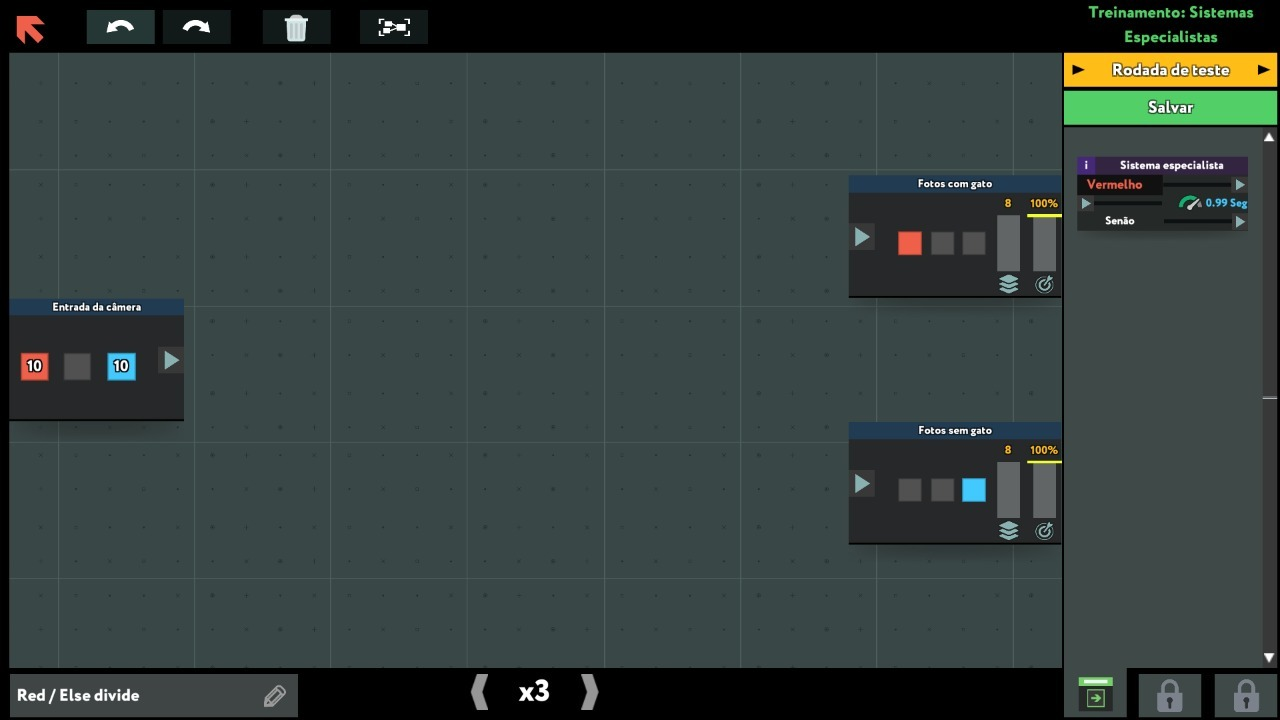
\includegraphics[width=0.9\textwidth]{fase}
    \fonte{\citeonline{while-true-learn}}
\end{figure}

\newpage

Para fazer o jogo, será necessário entender alguns componentes essenciais.

\vspace{1em}

\begin{figure}[!h]
    \centering
    \legenda[fig:componentes-da-fase]{Componentes da fase}
    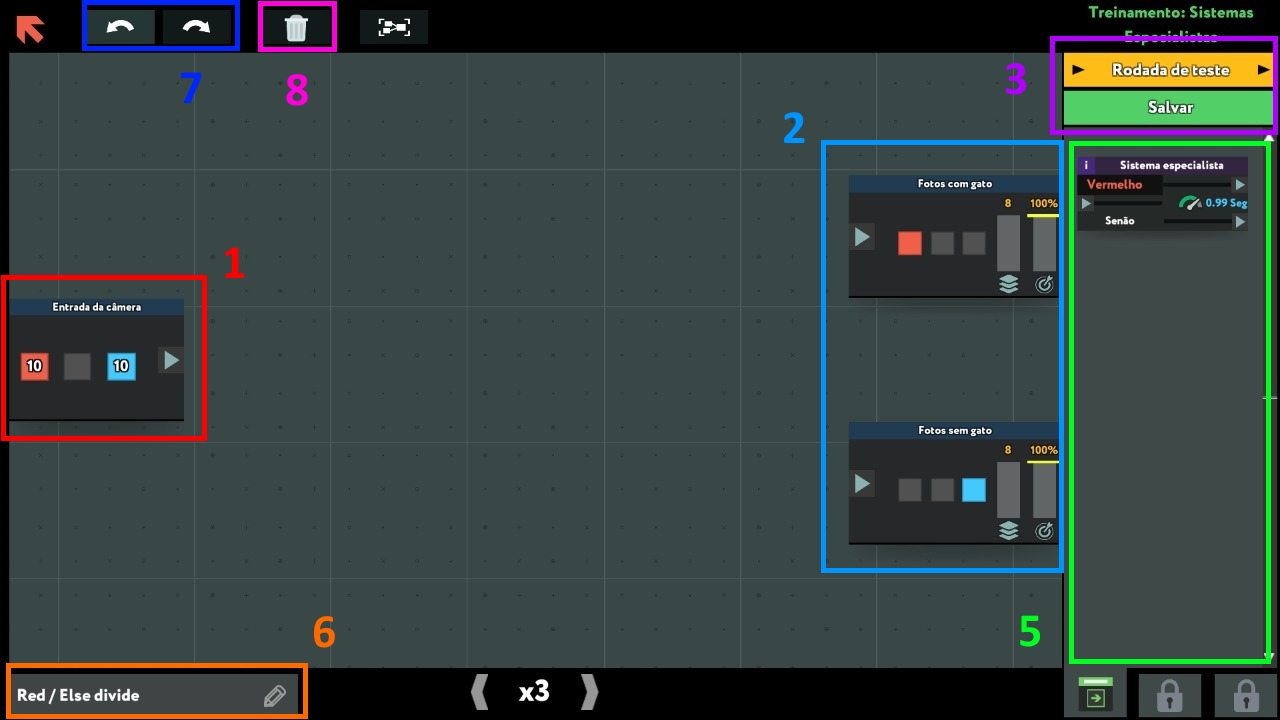
\includegraphics[width=0.9\textwidth]{componentes-da-fase}
    \fonte{\citeonline{while-true-learn}}
\end{figure}

\vspace{1em}

O componente 1 é a entrada que irá mandar um dado aleatório em seu armazenamento para a sua saída.

O componente 2 são as saídas que receberão os dados enviados para suas respectivas entradas.

O componente 3 são o botão que roda o programa e o botão que salva o esquema.

O componente 5 é onde estão guardados os nós que poderão ser arrastados para serem colocados no programa.

O componente 6 é o nome do esquema que poderá ser modificado.

O componente 7 é o botão de fazer e desfazer.

E o componente 8 é botão que deleta todos os nós utilizados.

% -----------------------------------------------------------------------
% -----------------------------------------------------------------------
\chapter{Histórico do jogo}
\label{cap:historico-do-jogo}

Histórico do jogo.

% -----------------------------------------------------------------------
% -----------------------------------------------------------------------
\chapter{Elementos de apoio}
\label{cap:apoio}

% -----------------------------------------------------------------------
\section{Ilustrações}
\label{cap:ilustracoes}

Ilustrações são elementos cuja função é complementar ao texto: são explicativas 
e informativas, não podendo apenas adornar ou enfeitar o trabalho. Fazem parte 
das ilustrações: desenhos, esquemas, fluxogramas, fotografias, gráficos, mapas, 
organogramas, plantas, quadros, retratos, figuras, imagens e outros.

A ilustração deve ser anunciada no texto – chamada pelo seu nmero (algarismos 
arábicos) – e inserida o mais próximo possível do trecho a que se refere.
Qualquer que seja o tipo de ilustração, sua identificação aparece na parte 
superior, precedida da palavra designativa (Figura, Mapa, Gráfico, etc.), 
seguida de seu número de ordem de ocorrência no texto, em algarismos arábicos, 
hífen ou travessão e do respectivo título.

Quando a ilustração for elaborada pelo(s) autor(es) do trabalho, deverá 
aparecer ``o próprio autor'' ou, no caso de trabalho em equipe, ``os próprios 
autores''. A \autoref{fig:grafico} apresenta um exemplo de gráfico. A 
\autoref{fig:figura} apresenta um exemplo de figura centralizada, enquanto a 
\autoref{fig:subfigura} apresenta exemplos de subfiguras.

\begin{grafico}[htb]
    \legenda[fig:grafico]{Exemplo de gráfico}
    \fig{scale=0.6}{imagens/teste}
    \fonte{\citeonline[p. 24]{araujo2012}}
\end{grafico}

\begin{figure}[htb]
    \legenda[fig:figura]{Exemplo de figura}
    \fig{scale=0.6}{imagens/teste}
    \fonte{\citeonline[p. 24]{araujo2012}}
\end{figure}

\begin{figure}[htb]
    \legenda[fig:subfigura]{Exemplo de várias subfiguras}
    \sfig{scale=0.3}{imagens/teste}\hfil
    \sfig{scale=0.3}{imagens/teste}\hfil
    \sfig{scale=0.3}{imagens/teste}
    
    \lfig[s:a3]{scale=0.3}{imagens/teste}{zzzz}\hfil
    \lfig[s:a3]{scale=0.3}{imagens/teste}{zzzz}\hfil
    \lfig[s:a4]{scale=0.3}{imagens/teste}{yyyy}
    
    \fonte{teste}
\end{figure}

% -----------------------------------------------------------------------
\section{Tabelas e Quadros}
\label{sec:tabelas}

As tabelas não são consideradas ilustrações, mas, sim, elementos demonstrativos 
de síntese. Por serem autossuficientes, não complementam o texto, isto porque 
já fazem parte dele como uma organização estrutural esquematizada. Segundo o 
IBGE (1993), as tabelas apresentam dados e/ou informações oriundos de 
tratamento estatístico e sua inserção no decorrer dos trabalhos segue as mesmas 
regras aplicadas para as ilustrações (identificação na parte superior com 
número e título, e fonte de referência na parte inferior em letra menor).

As tabelas podem ser inseridas no texto ou em anexo (principalmente as de 
formato grande, que ocupam uma página inteira ou mais). Recomenda-se incluir a 
observação ``continua...'' e ``... continuação'' nas respectivas partes, quando 
a tabela ocupar mais de uma página. Quando inseridas no texto, devem ser 
alinhadas às margens laterais ou centralizadas, se apresentarem formato pequeno.

Em suas delimitações, são usados traços horizontais para destacar o cabeçalho, 
bem como traço horizontal final. Indica-se a delimitação, no alto e em baixo, 
por traços horizontais grossos, preferencialmente. Não deve ser delineada à 
direita e à esquerda, por traços verticais e é facultativo o emprego de traços 
verticais para separação das colunas no corpo da tabela.

Teste %\citealias{abntex2-wiki-como-customizar}
%\citeasnoun{abntex2-wiki-como-customizar}
%\cites{abntex2-wiki-como-customizar}
%\citename

\cite{abntex2cite}

\citeonline{abntex2cite}



\begin{table}[htb]
    \legenda[tab:exemplo]{Exemplo de tabela}
    \begin{tabular}{c|ccc}
        \hline\
        \textbf{Pessoa} & \textbf{Idade} & \textbf{Peso} & \textbf{Altura} \\ 
        \hline\hline
        Marcos & 26    & 68   & 178    \\ 
        Ivone  & 22    & 57   & 162    \\ 
        ...    & ...   & ...  & ...    \\ 
        Sueli  & 40    & 65   & 153    \\ \hline
    \end{tabular}
    
    \fonteautor
\end{table}
 
Quando houver informações ou dados numéricos que não necessitem de cálculos 
(por exemplo, características, propriedades, relações, etc.), poderão ser 
utilizados os quadros. Nestes, os traços contornam toda a tabela.

\begin{lista}
	\item novo
	\item asd
	\item asd
	\item asd
	\item asd
\end{lista}

\begin{quadro}[htb]
    \legenda[quadro:exemplo]{Exemplo de quadro}
    \begin{tabular}{|c||c|c|c|}
        \hline
        \textbf{Pessoa} & \textbf{Idade} & \textbf{Peso} & \textbf{Altura} \\ 
        \hline\hline
        Marcos & 26    & 68   & 178    \\ \hline
        Ivone  & 22    & 57   & 162    \\ \hline
        ...    & ...   & ...  & ...    \\ \hline
        Sueli  & 40    & 65   & 153    \\ \hline
    \end{tabular}
    
    \fonte{\citeauthor{EIA649B}}
\end{quadro}

% -----------------------------------------------------------------------
\section{Equações}
\label{sec:equações}

Para facilitar a leitura, equações e fórmulas devem ser destacadas no texto e, 
se necessário, numeradas com algarismos arábicos entre parênteses, alinhados à 
direita. Na sequência normal do texto, é permitido o uso de uma entrelinha 
maior que comporte seus elementos (expoentes, índices, entre outros). A 
\autoref{eq:exemplo} apresenta um exemplo de equação.

\begin{equation}
\label{eq:exemplo}
C_{(A,B)} = \{ p \in
A\;|\;[(\overrightarrow{q_i-c}){\cdot}{\vec{n}}_c][(\overrightarrow{q_j-c})
{\cdot}{\vec{n}}_c]
< 0 \}
\end{equation}

% -----------------------------------------------------------------------
% -----------------------------------------------------------------------
\section{Códigos e Algoritmos}
\label{sec:codigos}

Os códigos e algoritmos podem ser inseridos no texto usando comandos 
\texttt{codigo} e \texttt{algoritmo}, respectivamente. O \autoref{cod:fib} 
apresenta um exemplo de código em C.

\begin{codigo}[htb]
    \legenda[cod:fib]{Calcula Fibonacci}
    \begin{lstlisting}[language=C]
    int main() {
        int n, first = 0, second = 1, next, c;
        
        printf("Enter the number of terms\n");
        scanf("%d", &n);
        
        printf("First %d terms of Fibonacci series are :-\n", n);
        
        for (c = 0; c < n; c++){
            if (c <= 1) next = c;
            else {
                next = first + second;
                first = second;
                second = next;
            }
            printf("%d\n",next);
        }
        
        return 0;
    }
    \end{lstlisting}
    
    \fonteautor
\end{codigo}


% -----------------------------------------------------------------------
% -----------------------------------------------------------------------
\chapter{Conclusão}

É a parte final do trabalho, na qual se apresentam as conclusões 
correspondentes aos objetivos e às hipóteses: informa se os objetivos foram 
alcançados ou não – seguidos de justificativas e explicações caso os mesmos não 
tenham sido alcançados – bem como se as hipóteses foram negadas ou 
corroboradas. É possível que se apresentem também:

\begin{lista}
    \item comentários relativos aos resultados obtidos, fechando o raciocínio 
    por meio de um processo dedutivo,
    
    \item a importância dos resultados obtidos,
    
    \item a projeção da pesquisa, com estimativas para o uso dos resultados,
    
    \item a repercussão, informando quem será beneficiado e em quê,
    
    \item as limitações do trabalho, mostrando suas fragilidades ou
insuficiências,
    \item as dificuldades encontradas no decorrer da pesquisa, e
    \item indicações para trabalhos futuros, para a continuidade da
pesquisa pelo próprio autor e por outros. Teste
\end{lista}

Veja \autoref{apendice:teste}.

% ----------------------------------------------------------
% ELEMENTOS PÓS-TEXTUAIS
% ----------------------------------------------------------
%\postextual
% ----------------------------------------------------------

% ----------------------------------------------------------
% Referências bibliográficas
% ----------------------------------------------------------
\bibliography{referencias}

% ----------------------------------------------------------
% Apêndices
% ----------------------------------------------------------
% Material complementar preparado pelo autor
\apendice[apendice:teste]{TESTE}

% ----------------------------------------------------------
% Anexos
% ----------------------------------------------------------
% Material complementar nao preparado pelo autor
\anexo[apendice:teste1]{TESTE}


\end{document}
